To develop a suitable model based controller, the developed non-linear model should first be validate. This is done using a planar 2 degree-of-freedom soft robot. This robot has a translational and rotational degree of freedom. Rotation is only dependent on the difference in bellow length, not absolute bellow length. To measure rotation, an Inertial Measurement Unit (IMU) is connected at the tip of the robot. The position of the bellows can be tracked with an optical tracking system. From this data, elongation and curvature of each individual bellow can extracted. This allows validation of the dynamic model.


\section{Control Architecture}


\subsection{Inertial Measurement Unit (IMU)}

The IMU will be used to determine actuator's rotation. The Mahony-Madgwick filter as used by Berkers might be implemented. If available, a library can be downloaded which does the sensor fusion by itself. The IMU will measure rotation either in degrees or radians which should be converted to a curvature. To convert the angle to curvature the actual length of the actuator should also be known. This will be determined using a image tracking vision system.

\subsection{Vision system}

The vision system Pixy2 can track objects. A marker connected to the tip of the actuator will be tracked. To my best knowledge this measures absolute place of the marker. Pure elongation won't be a problem to measure. However, problems arise for determining curvature and elongation. Since $\phi = \kappa l$, any combination between $\kappa$ and $l = L_0\epsilon$ is possible. Hence, the elongation can not be determined that easily. 

\subsection{Pressure sensor}






\todo{include hardware list}



\section{Simulation model}

A simplified dynamic model is derived in an effort to capture the dynamics of the soft manipulator. It is assumed that the dynamics of the system can be formulated as, 

\begin{equation}
    M(q)\Ddot{q} + C\dot{q} + K(q)q = u \hspace{10pt} \text{with} \hspace{10pt} u = Hp
\end{equation}

which resembles a non-linear mass-spring-damper system. Here, $M(q)  \in \mathbb{R}^{n\times n}$ is a non-linear mass matrix, $C   \in \mathbb{R}^{n\times n}$ a linear damping matrix, and $K(q)   \in \mathbb{R}^{n\times n}$ a non-linear stiffness matrix. Matrix $H   \in \mathbb{R}^{2\times 2}$ maps input pressure $p$ to forces and moments $u$.

Above dynamic model allows for numeric solving by reformulating the model to a second order state-space formulation as,

\begin{equation}
     \begin{bmatrix} \dot{x}  \end{bmatrix}   =      \begin{bmatrix} O_2 & I_2 \\ -M(q)^{-1}K(q)  & -M(q)^{-1} C \end{bmatrix}      \begin{bmatrix} x \end{bmatrix}  +      \begin{bmatrix} O_2 \\ M(q)^{-1}H   \end{bmatrix}       \begin{bmatrix} p_1\\ p_2   \end{bmatrix} 
\end{equation}

where $x \in \mathbb{R}^{n}$ is the state vector. Assuming the constant curvature approach ($n = 2$) the entries of of $x$ are $ \begin{bmatrix} \epsilon \hspace{3pt} \kappa \hspace{3pt} \dot{\epsilon}  \hspace{3pt} \dot{\kappa}  \end{bmatrix}^{\top}  $



\subsection{Inverse Kinematics}


\begin{figure}[H]
    \centering
    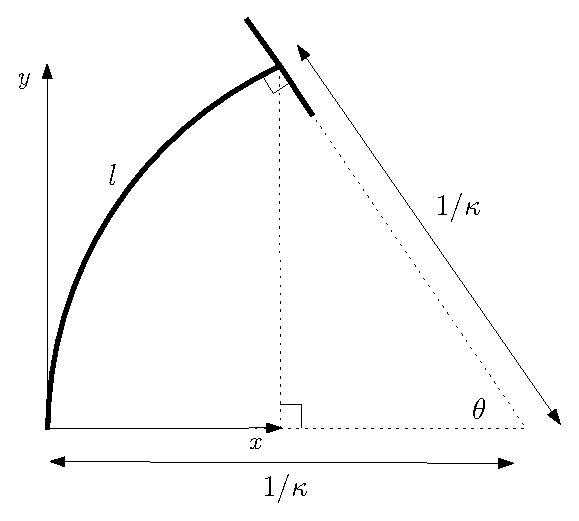
\includegraphics[width = 0.5\textwidth]{Figures/Chapter5/fbdkinematics.eps}
    \caption{Schematic drawing of the actuator to determine mapping from configuration space to task space}
    \label{fig:my_label}
\end{figure}


\begin{equation}
    \theta = l \kappa
\end{equation}


\begin{equation}
    y = \frac{1}{\kappa}\sin(l \kappa)
\end{equation}

\begin{equation}
    x = \frac{1}{\kappa}[1-\cos(l \kappa)]
\end{equation}





\textbf{Assumptions}
\begin{itemize}
    \item The actuator is symmetrical, curvature equal but negative in when bellow is pressurized
    \item Out of plane motion is negligible small
    \item Constant curvature approach captures the kinematics well when neglecting the effect of gravity 
\end{itemize}



